\documentclass[14 pt,xcolor=dvipsnames]{beamer}

\usepackage{epsdice}

\usepackage[absolute,overlay]{textpos}

\usepackage[orientation=portrait,size=custom,width=25.4,height=19.05]{beamerposter}

%25,4 см 19,05 см размеры слайда в powerpoint

\usetheme{metropolis}
\metroset{
  %progressbar=none,
  numbering=none,
  subsectionpage=progressbar,
  block=fill
}

%\usecolortheme{seahorse}

\usepackage{fontspec}
\usepackage{polyglossia}
\setmainlanguage{russian}


\usepackage{fontawesome5} % removed [fixed]
\setmainfont[Ligatures=TeX]{Myriad Pro}
\setsansfont{Myriad Pro}


\usepackage{amssymb,amsmath,amsxtra,amsthm}


\usepackage{unicode-math}
\usepackage{centernot}

\usepackage{graphicx}
\graphicspath{{img/}}

\usepackage{wrapfig}
\usepackage{animate}
\usepackage{tikz}
%\usetikzlibrary{shapes.geometric,patterns,positioning,matrix,calc,arrows,shapes,fit,decorations,decorations.pathmorphing}
\usepackage{pifont}
\usepackage{comment}
\usepackage[font=small,labelfont=bf]{caption}
\captionsetup[figure]{labelformat=empty}
\includecomment{techno}

\usefonttheme[onlymath]{serif}


%Расположение

\setbeamersize{text margin left=15 mm,text margin right=5mm} 
\setlength{\leftmargini}{38 pt}

%\usepackage{showframe}
%\usepackage{enumitem}
%\setlist{leftmargin=5.5mm}


%Цвета от дирекции

\definecolor{dirblack}{RGB}{58, 58, 58}
\definecolor{dirwhite}{RGB}{245, 245, 245}
\definecolor{dirred}{RGB}{149, 55, 53}
\definecolor{dirblue}{RGB}{0, 90, 171}
\definecolor{dirorange}{RGB}{235, 143, 76}
\definecolor{dirlightblue}{RGB}{75, 172, 198}
\definecolor{dirgreen}{RGB}{155, 187, 89}
\definecolor{dircomment}{RGB}{128, 100, 162}

\setbeamercolor{title separator}{bg=dirlightblue!50, fg=dirblue}

%Цвета блоков

\setbeamercolor{block title}{bg=dirblue!30,fg=dirblack}

\setbeamercolor{block title example}{bg=dirlightblue!50,fg=dirblack}

\setbeamercolor{block body example}{bg=dirlightblue!20,fg=dirblack}

\AtBeginEnvironment{exampleblock}{\setbeamercolor{itemize item}{fg=dirblack}}
%\setbeamertemplate{blocks}[rounded][shadow]

% Набор команд для удобства верстки

\newcommand{\RR}{\mathbb{R}}
\newcommand{\ZZ}{\mathbb{Z}}
\newcommand{\la}{\lambda}

% Набор команд для структуризации

%\newcommand{\quest}{\faQuestionCircleO}
%\faPencilSquareO \faPuzzlePiece \faQuestionCircleO  \faIcon*[regular]{file} {\textcolor{dirblue}
%\newcommand{\quest}{\textcolor{dirblue}{\boxed{\textbf{?}}}
\newcommand{\task}{\faIcon{tasks}}
\newcommand{\exmpl}{\faPuzzlePiece}
\newcommand{\dfn}{\faIcon{pen-square}}
\newcommand{\quest}{\textcolor{dirblue}{\faQuestionCircle[regular]}}
\newcommand{\acc}[1]{\textcolor{dirred}{#1}}
\newcommand{\accm}[1]{\textcolor{dirred}{#1}}
\newcommand{\acct}[1]{\textcolor{dirblue}{#1}}
\newcommand{\acctm}[1]{\textcolor{dirblue}{#1}}
\newcommand{\accex}[1]{\textcolor{dirblack}{\bf #1}}
\newcommand{\accexm}[1]{\textcolor{dirblack}{ \mathbf{#1}}}
\newcommand{\acclp}[1]{\textcolor{dirorange}{\it #1}}


\newcommand{\videotitle}[1]{\begin{center}
    \textcolor{dirblue}{#1}

    \todo{название видеофрагмента}
\end{center}}

\newcommand{\lecturetitle}[1]{\begin{center}
    \textcolor{dirblue}{#1}

    \todo{название лекции}
\end{center}}




\newcommand{\todo}[1]{\textcolor{dircomment}{\bf #1}}

\newcommand{\spcbig}{\vspace{-10 pt}}
\newcommand{\spcsmall}{\vspace{-5 pt}}

%\usepackage{listings}
%\lstset{
%xleftmargin=0 pt,
%  basicstyle=\small, 
%  language=Python,
  %tabsize = 2,
%  backgroundcolor=\color{mc!20!white}
%}



%\newcommand{\mypart}[1]{\begin{frame}[standout]{\huge #1}\end{frame}}

\setbeamercolor{background canvas}{bg=}

% frame title setup
\setbeamercolor{frametitle}{bg=,fg=dirblue}
\setbeamertemplate{frametitle}[default][left]

\addtobeamertemplate{frametitle}{\hspace*{-0.5 cm}}{\vspace*{0.25cm}}


%Шрифты
\setbeamerfont{frametitle}{family=\rmfamily,series=\bfseries,size={\fontsize{33}{30}}}
\setbeamerfont{framesubtitle}{family=\rmfamily,series=\bfseries,size={\fontsize{26}{20}}}





\usepackage{physics}
\newcommand{\R}{\mathbb{R}}

\usepackage[outline]{contour}




\usepackage{pgfplots}
\pgfplotsset{compat=newest}

\usepackage{tikz}
\usetikzlibrary{calc}
\usetikzlibrary{quotes,angles}
\usetikzlibrary{arrows}
\usetikzlibrary{arrows.meta}
\usetikzlibrary{positioning,intersections,decorations.markings}
\usetikzlibrary{patterns}

\usepackage{tkz-euclide} 

\newcommand{\grid}{\draw[color=gray,step=1.0,dotted] (-2.1,-2.1) grid (9.6,6.1)}

\newcommand{\ba}{\symbf{a}}
\newcommand{\bb}{\symbf{b}}
\newcommand{\bc}{\symbf{c}}
\newcommand{\bd}{\symbf{d}}
\newcommand{\bx}{\symbf{x}}
\newcommand{\bv}{\symbf{v}}
\newcommand{\Lin}{\mathrm{Lin}}


%\tikzset{>=latex}

\colorlet{veca}{red}
\colorlet{vecb}{blue}
\colorlet{vecc}{olive}








\begin{document}

% \maketitle


\begin{frame} % название лекции


\lecturetitle{Векторы и операторы}

\end{frame}


% !TEX root = ../linal_lecture_01.tex

\begin{frame} % название фрагмента

\videotitle{Вектор: длина и скалярное произведение}

\end{frame}




\begin{frame}{Краткое напутствие}

%\uncover<1->{
    Зачем нужна \alert{линейная алгебра}?

\begin{itemize}[<+->]
  \item Линейная алгебра прекрасна сама по себе!
  \item Работает «под капотом» практически всех методов машинного обучения.
\end{itemize}

%}
\end{frame}



\begin{frame}{Краткий план:}
  \begin{itemize}[<+->]
    \item Вектор — это столбец чисел.
    \item Сложение двух векторов и умножение на число.
    \item Расстояние и косинус угла между векторами.
  \end{itemize}

\end{frame}


\begin{frame}{Вектор}


\begin{itemize}[<+->]
\item Рабочее определение. 

\alert{Вектор} — столбец из нескольких чисел.   

\[
\bv = \begin{pmatrix}
  \sqrt{5} \\
  3 \\
  -3.45
\end{pmatrix}
\]

\item Идея вектора. Вектор — всё, что можно описать столбцом из нескольких чисел. 

\item Мы не пишем стрелочку над вектором.

\item Вектор из нулей обозначаем $\bzero$.

\end{itemize}

\end{frame}



\begin{frame}{Пространство $\R^n$}

\begin{itemize}[<+->]
  \item Определение. \alert{Пространство $\R^n$:}

     Множество всех возможных векторов из $n$ чисел. 
 \[
 \R^n = \left\{ \begin{pmatrix}
 x_1 \\
 x_2 \\
 \vdots \\
 x_n \\
 \end{pmatrix} \middle| x_1 \in \R, \ldots, x_n \in \R
   \right\}  
 \]

\item Определение. \alert{Размерность} пространства $\R^n$:

    Количество чисел в каждом векторе, $n$.
\end{itemize}
\end{frame}







\begin{frame}{Длина вектора}




\begin{minipage}{0.3\textwidth}% adapt widths of minipages to your needs
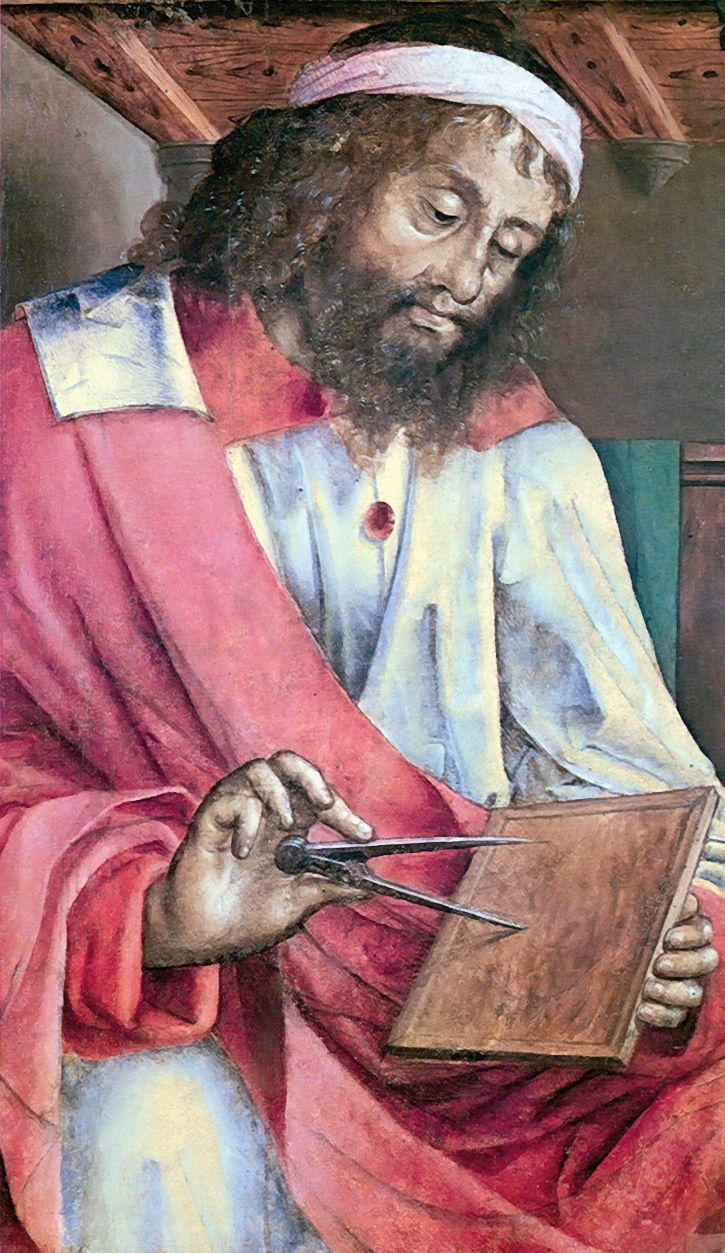
\includegraphics[scale=0.2]{figures/video_010_euklid.jpg}
\end{minipage}%
\hfill%
\begin{minipage}{0.6\textwidth}
Определение. 

\alert{Евклидова длина} или \alert{норма} вектора 

$\norm{\bx} = \sqrt{x_1^2 + x_2^2 + \ldots + x_n^2}$.
\end{minipage}

\figcaption{Евклид, около 300 лет до н.э.}

\graylink{wikipedia.org / общественное достояние}



\end{frame}



\begin{frame}
\begin{tikzpicture}[
scale=1.6,
MyPoints/.style={draw=blue,fill=white,thick},
Segments/.style={draw=blue!50!red!70,thick},
MyCircles/.style={green!50!blue!50,thin}, 
every node/.style={scale=1}
]
\grid;
\clip (-2.5,-2.5) rectangle (10.5,6.5);


%\draw[->, >=stealth] (-1,0)--(6.5,0) node[right]{$x_1$};
\draw[-{Latex[length=4.5mm, width=2.5mm]}, >=stealth] (0,-1)--(0,5) node[above left]{$x_2$};

\draw[-{Latex[length=4.5mm, width=2.5mm]}, >=stealth] (-1,0)--(6.5,0) 
node[right]{$x_1$};


%{\verb!->!new, arrowhead = 2mm, line width=4pt}
%, arrowhead = 3mm
%, arrowhead = 0.2

% Feel free to change here coordinates of points A and B
\pgfmathparse{0}		\let\Xa\pgfmathresult
\pgfmathparse{0}		\let\Ya\pgfmathresult
\coordinate (A) at (\Xa,\Ya);

\pgfmathparse{4}		\let\Xb\pgfmathresult
\pgfmathparse{3}		\let\Yb\pgfmathresult
\coordinate (B) at (\Xb,\Yb);

\pgfmathparse{4}		\let\Xc\pgfmathresult
\pgfmathparse{0}		\let\Yc\pgfmathresult
\coordinate (C) at (\Xc,\Yc);


% Let I be the midpoint of [AB]
\pgfmathparse{(\Xb+\Xa)/2} \let\XI\pgfmathresult
\pgfmathparse{(\Yb+\Ya)/2} \let\YI\pgfmathresult
\coordinate (I) at (\XI,\YI);	


\draw[-{Latex[length=4.5mm, width=2.5mm]}, >=stealth, vecb,thick] (A)--(B) node[midway,above]{$\bx$};

\draw[black, dashed, thick] (B)--(C) node[midway,right]{$3$};

\draw[black] (A)--(C) node[midway,below]{$4$};

\tkzMarkRightAngle[size=.3](A,C,B) 

\node [above right,darkgray] at (1,3.5) {$\bx=\left(\begin{array}{l}4 \\ 3\end{array}\right) \quad \|\bx\|=\sqrt{3^{2}+4^{2}}=5 $};

\end{tikzpicture}



\end{frame}




\begin{frame}{Сложение и вычитание двух векторов}

 Определение. \alert{Сложение и вычитание} двух векторов выполняем поэлементно:
    \[
    \begin{pmatrix}
      2 \\
      3.5 \\
      -1 
    \end{pmatrix} + \begin{pmatrix}
      3 \\
      -3 \\
      1 
    \end{pmatrix}  = \begin{pmatrix}
      5 \\
      0.5 \\
      0 
    \end{pmatrix}
    \]  


\begin{tikzpicture}[
scale=1.2,
MyPoints/.style={draw=blue,fill=white,thick},
Segments/.style={draw=blue!50!red!70,thick},
MyCircles/.style={green!50!blue!50,thin}, 
every node/.style={scale=1.2}
]
%\grid;
%\clip (-.5,-.5) rectangle (5.5,5.5);


%%\draw[->, >=stealth] (-1,0)--(6.5,0) node[right]{$x_1$};
%\draw[-{Latex[length=4.5mm, width=2.5mm]}, >=stealth] (0,-1)--(0,5) node[above left]{$x_2$};
%
%\draw[-{Latex[length=4.5mm, width=2.5mm]}, >=stealth] (-1,0)--(6.5,0) 
%node[right]{$x_1$};

% Feel free to change here coordinates of points A and B
\pgfmathparse{0}		\let\Xa\pgfmathresult
\pgfmathparse{0}		\let\Ya\pgfmathresult
\coordinate (A) at (\Xa,\Ya);

\pgfmathparse{2}		\let\Xb\pgfmathresult
\pgfmathparse{4}		\let\Yb\pgfmathresult
\coordinate (B) at (\Xb,\Yb);

\pgfmathparse{3}		\let\Xc\pgfmathresult
\pgfmathparse{1}		\let\Yc\pgfmathresult
\coordinate (C) at (\Xc,\Yc);

\pgfmathparse{5}		\let\Xd\pgfmathresult
\pgfmathparse{5}		\let\Yd\pgfmathresult
\coordinate (D) at (\Xd,\Yd);



% Let I be the midpoint of [AB]
\pgfmathparse{(\Xb+\Xa)/2} \let\XI\pgfmathresult
\pgfmathparse{(\Yb+\Ya)/2} \let\YI\pgfmathresult
\coordinate (I) at (\XI,\YI);	


\draw[-{Latex[length=4.5mm, width=2.5mm]}, >=stealth, vecb,thick] (A)--(B) node[midway,left]{$\ba$};

\draw[-{Latex[length=4.5mm, width=1.5mm]}, >=stealth, vecb,dashed] (C)--(D) node[midway,right]{$\ba$};


\draw[-{Latex[length=4.5mm, width=2.5mm]}, >=stealth, veca,thick] (A)--(C) node[midway,below]{$\bb$};

\draw[-{Latex[length=4.5mm, width=1.5mm]}, >=stealth, veca,dashed] (B)--(D) node[midway,above]{$\bb$};


\draw[-{Latex[length=4.5mm, width=2.5mm]}, >=stealth, vecc,thick] (A)--(D) node[midway,above, sloped]{$\ba+\bb$};


\end{tikzpicture}


\end{frame}



\begin{frame}{Умножение вектора на число}


Определение. \alert{Умножение} вектора на число выполняем поэлеметно:
    \[
    4 \cdot \begin{pmatrix}
      2 \\
      3.5 \\
      -1 
    \end{pmatrix} = \begin{pmatrix}
      8 \\
      14 \\
      -4 
    \end{pmatrix}  
    \]



\begin{tikzpicture}[
  scale=1.2,
  MyPoints/.style={draw=blue,fill=white,thick},
  Segments/.style={draw=blue!50!red!70,thick},
  MyCircles/.style={green!50!blue!50,thin}, 
  every node/.style={scale=1.2}
  ]
  %\grid;
  %\clip (-.5,-.5) rectangle (5.5,5.5);

  \pgfmathparse{0}		\let\Xa\pgfmathresult
  \pgfmathparse{0}		\let\Ya\pgfmathresult
  \coordinate (A) at (\Xa,\Ya);

  \pgfmathparse{3}		\let\Xb\pgfmathresult
  \pgfmathparse{3}		\let\Yb\pgfmathresult
  \coordinate (B) at (\Xb,\Yb);

  \pgfmathparse{5}		\let\Xc\pgfmathresult
  \pgfmathparse{5}		\let\Yc\pgfmathresult
  \coordinate (C) at (\Xc,\Yc);

  \draw[-{Latex[length=4.5mm, width=2.5mm]}, >=stealth, black,thick] (A)--(C) node[above left]{$\lambda \cdot \ba$};

  \draw[-{Latex[length=4.5mm, width=2.5mm]}, >=stealth, veca,thick] (A)--(B) node[midway,above left]{$\ba$};


  \end{tikzpicture}


\end{frame}




\begin{frame}{Расстояние между векторами}

Определение. \alert{Евклидово расстояние} между векторами
  \[
  d(\ba, \bb) = \norm{\ba - \bb} = \sqrt{(a_1 - b_1)^2 + \ldots + (a_n - b_n)^2}
  \]

\begin{itemize}
  \item по определению, $d(\ba, \bb) \geq 0$. 
  \item также говорят \alert{Евклидова метрика}
\end{itemize}


\begin{tikzpicture}[
scale=1.2,
MyPoints/.style={draw=blue,fill=white,thick},
Segments/.style={draw=blue!50!red!70,thick},
MyCircles/.style={green!50!blue!50,thin}, 
every node/.style={scale=1.2}
]
%\grid;
%\clip (-.5,-.5) rectangle (5.5,5.5);


%%\draw[->, >=stealth] (-1,0)--(6.5,0) node[right]{$x_1$};
%\draw[-{Latex[length=4.5mm, width=2.5mm]}, >=stealth] (0,-1)--(0,5) node[above left]{$x_2$};
%
%\draw[-{Latex[length=4.5mm, width=2.5mm]}, >=stealth] (-1,0)--(6.5,0) 
%node[right]{$x_1$};

% Feel free to change here coordinates of points A and B
\pgfmathparse{0}		\let\Xa\pgfmathresult
\pgfmathparse{0}		\let\Ya\pgfmathresult
\coordinate (A) at (\Xa,\Ya);

\pgfmathparse{1}		\let\Xb\pgfmathresult
\pgfmathparse{4}		\let\Yb\pgfmathresult
\coordinate (B) at (\Xb,\Yb);

\pgfmathparse{3}		\let\Xc\pgfmathresult
\pgfmathparse{1}		\let\Yc\pgfmathresult
\coordinate (C) at (\Xc,\Yc);




% Let I be the midpoint of [AB]
\pgfmathparse{(\Xb+\Xa)/2} \let\XI\pgfmathresult
\pgfmathparse{(\Yb+\Ya)/2} \let\YI\pgfmathresult
\coordinate (I) at (\XI,\YI);	


\draw[-{Latex[length=4.5mm, width=2.5mm]}, >=stealth, vecb,thick] (A)--(B) node[midway,left]{$\ba$};


\draw[-{Latex[length=4.5mm, width=2.5mm]}, >=stealth, veca,thick] (A)--(C) node[midway,below]{$\bb$};


\draw[-{Latex[length=4.5mm, width=2.5mm]}, >=stealth, vecc,thick] (C)--(B) node[midway,right]{$\ba-\bb$};


\end{tikzpicture}
    


\end{frame}






\begin{frame}{Скалярное произведение и угол}

\begin{itemize}[<+->]
\item Определение. \alert{Скалярное произведение} векторов $\ba$ и $\bb$:
  $\langle \ba, \bb \rangle = a_1 b_1 + a_2 b_2 + \ldots + a_n b_n$.

\item Определение. 
\alert{Косинус угла} и \alert{угол} между векторами $\ba$ и $\bb$:
% Косинусная близость, cosine similarity:  
  \[
  \cos \angle (\ba, \bb) =  \frac{\langle \ba, \bb \rangle}{ \norm{\ba} \norm{\bb}} \quad   \angle (\ba, \bb) =  \arccos \frac{\langle \ba, \bb \rangle}{ \norm{\ba} \norm{\bb}} 
  \]
\end{itemize}

\begin{tikzpicture}[
scale=1.2,
MyPoints/.style={draw=blue,fill=white,thick},
Segments/.style={draw=blue!50!red!70,thick},
MyCircles/.style={green!50!blue!50,thin}, 
every node/.style={scale=1.2}
]
%\grid;

%\clip (-.5,-.5) rectangle (6.5,5.5);


%%\draw[->, >=stealth] (-1,0)--(6.5,0) node[right]{$x_1$};
%\draw[-{Latex[length=4.5mm, width=2.5mm]}, >=stealth] (0,-1)--(0,5) node[above left]{$x_2$};
%
%\draw[-{Latex[length=4.5mm, width=2.5mm]}, >=stealth] (-1,0)--(6.5,0) 
%node[right]{$x_1$};

% Feel free to change here coordinates of points A and B
\pgfmathparse{0}		\let\Xa\pgfmathresult
\pgfmathparse{0}		\let\Ya\pgfmathresult
\coordinate (A) at (\Xa,\Ya);

\pgfmathparse{1}		\let\Xb\pgfmathresult
\pgfmathparse{4}		\let\Yb\pgfmathresult
\coordinate (B) at (\Xb,\Yb);

\pgfmathparse{4}		\let\Xc\pgfmathresult
\pgfmathparse{1}		\let\Yc\pgfmathresult
\coordinate (C) at (\Xc,\Yc);


\draw[-{Latex[length=4.5mm, width=2.5mm]}, >=stealth, vecb,thick] (A)--(B) node[midway,left]{$\ba$};


\draw[-{Latex[length=4.5mm, width=2.5mm]}, >=stealth, veca,thick] (A)--(C) node[midway,below]{$\bb$};


\tkzMarkAngle[size=1, mark = none](C,A,B);

\node [darkgray] at (1,1) {$\varphi$}; 

% \node [above right, darkgray] at (2, 2) {$\cos \varphi=\dfrac{\langle \ba, \bb\rangle}{\|\ba\| \cdot\|\bb\|}$}; 

%\draw
%(3,-1) coordinate (a) node[right] {$a$}
%-- (0,0) coordinate (b) node[left] {b}
%-- (2,2) coordinate (c) node[above right] {c}


\end{tikzpicture}
  
Угол определён, если $\norm{\ba} > 0$ и $\norm{\bb} > 0$.


\end{frame}



\begin{frame}{Скалярное произведение и проекция}

  Если вектор $\ba$ имеет единичную длину, $\norm{\ba} = 1$, то 


  $\langle \ba, \bb \rangle = \norm{\bb} \cos \phi$ — длина$^*$ проекции $b$ на $a$.
  

\begin{tikzpicture}[
scale=1.2,
MyPoints/.style={draw=blue,fill=white,thick},
Segments/.style={draw=blue!50!red!70,thick},
MyCircles/.style={green!50!blue!50,thin}, 
every node/.style={scale=1.2}
]
%\grid;

%\clip (-1.5,-1.5) rectangle (7.5,5.5);


%%\draw[->, >=stealth] (-1,0)--(6.5,0) node[right]{$x_1$};
%\draw[-{Latex[length=4.5mm, width=2.5mm]}, >=stealth] (0,-1)--(0,5) node[above left]{$x_2$};
%
%\draw[-{Latex[length=4.5mm, width=2.5mm]}, >=stealth] (-1,0)--(6.5,0) 
%node[right]{$x_1$};

% Feel free to change here coordinates of points A and B
\pgfmathparse{0}		\let\Xa\pgfmathresult
\pgfmathparse{0}		\let\Ya\pgfmathresult
\coordinate (A) at (\Xa,\Ya);

\pgfmathparse{5.5}		\let\Xb\pgfmathresult
\pgfmathparse{5.5}		\let\Yb\pgfmathresult
\coordinate (B) at (\Xb,\Yb);

\pgfmathparse{5}		\let\Xc\pgfmathresult
\pgfmathparse{2}		\let\Yc\pgfmathresult
\coordinate (C) at (\Xc,\Yc);

\pgfmathparse{-1}		\let\Xd\pgfmathresult
\pgfmathparse{1}		\let\Yd\pgfmathresult
\coordinate (D) at (\Xd,\Yd);

\pgfmathparse{3}		\let\Xe\pgfmathresult
\pgfmathparse{5}		\let\Ye\pgfmathresult
\coordinate (E) at (\Xe,\Ye);

\pgfmathparse{-0.75}		\let\Xf\pgfmathresult
\pgfmathparse{0.75}		\let\Yf\pgfmathresult
\coordinate (F) at (\Xf,\Yf);

\pgfmathparse{3.25}		\let\Xg\pgfmathresult
\pgfmathparse{4.75}		\let\Yg\pgfmathresult
\coordinate (G) at (\Xg,\Yg);

\pgfmathparse{4}		\let\Xh\pgfmathresult
\pgfmathparse{4}		\let\Yh\pgfmathresult
\coordinate (H) at (\Xh,\Yh);

\pgfmathparse{6}		\let\Xj\pgfmathresult
\pgfmathparse{2}		\let\Yj\pgfmathresult
\coordinate (J) at (\Xj,\Yj);

\draw[-{Latex[length=4.5mm, width=2.5mm]}, >=stealth, vecb,thick] (A)--(B) node[midway,left]{$\ba$};


\draw[-{Latex[length=4.5mm, width=2.5mm]}, >=stealth, veca,thick] (A)--(J) node[midway,below]{$\bb$};

\draw[thick] (A)--(D);
\draw[thick] (H)--(E);

\draw[thick, dashed] (J)--(E);


\draw[{Latex[length=4.5mm, width=2.5mm]}-{Latex[length=4.5mm, width=2.5mm]}, >=stealth, thick] (F)--(G) node[midway,above left]{$\langle \ba, \bb \rangle$};




\tkzMarkRightAngle[size=0.3, mark = none](A,H,J);

\tkzMarkAngle[size=1, mark = none](C,A,B);


%\node [below, darkgray] at (1,1) {$\varphi$}; 

%\node [below right, darkgray] at (-1.5,-1) {если  $\| \ba \| = 1 $, то $\langle \ba, \bb \rangle$  -- длина* проекции $\bb$ на $\ba$}; 



%\draw
%(3,-1) coordinate (a) node[right] {$a$}
%-- (0,0) coordinate (b) node[left] {b}
%-- (2,2) coordinate (c) node[above right] {c}


\end{tikzpicture}




\end{frame}


\begin{frame}{Свойства скалярного произведения}

  
  \begin{itemize}[<+->]
  \item Скалярное вектора на себя равно квадрату длины
  $\langle \ba, \ba \rangle = \norm{\ba}^2$

  \item Линейность по каждому аргументу
  $\langle \lambda \ba, \bb \rangle = \langle \ba,  \lambda  \bb \rangle = \lambda  \langle \ba,  \bb \rangle$

  $\langle \ba + \bb, \bc \rangle = \langle \ba , \bc \rangle + \langle \bb , \bc \rangle$

  \item Симметричность
  
  $\langle \ba, \bb \rangle = \langle \bb, \ba \rangle$
  \end{itemize}
  
  

\end{frame}





% \begin{frame}{Почти любой объект — вектор!}

%   \begin{block}{С помощью вектора можно закодировать:}
%   \begin{itemize}
%     \item многочлен 
%     \[
%     3x^2 + 6 x - 7 \to (3, 6, -7)  
%     \]
%     \item характеристики индивида

%     \[
%     \text{Блондин с ростом 182 см и весов 81 килограмм} \to (0, 182, 81)
%     \]
%     \item TODO
%   \end{itemize}

%   \end{block}
% \end{frame}




\begin{frame}{Ортогональность векторов}

Определение. Векторы $\ba$ и $\bb$ \alert{ортогональны}, $a\perp b$, если
\[
  \langle \ba, \bb \rangle =0
\]

Также говорят «\alert{перпендикулярны}».


\begin{tikzpicture}[
scale=1.8,
MyPoints/.style={draw=blue,fill=white,thick},
Segments/.style={draw=blue!50!red!70,thick},
MyCircles/.style={green!50!blue!50,thin}, 
every node/.style={scale=1.2}
]
%\grid;

\clip (-1.5,-1.5) rectangle (8.5,5.5);


%%\draw[->, >=stealth] (-1,0)--(6.5,0) node[right]{$x_1$};
%\draw[-{Latex[length=4.5mm, width=2.5mm]}, >=stealth] (0,-1)--(0,5) node[above left]{$x_2$};
%
%\draw[-{Latex[length=4.5mm, width=2.5mm]}, >=stealth] (-1,0)--(6.5,0) 
%node[right]{$x_1$};

% Feel free to change here coordinates of points A and B
\pgfmathparse{0}		\let\Xa\pgfmathresult
\pgfmathparse{0}		\let\Ya\pgfmathresult
\coordinate (A) at (\Xa,\Ya);

\pgfmathparse{1}		\let\Xb\pgfmathresult
\pgfmathparse{4}		\let\Yb\pgfmathresult
\coordinate (B) at (\Xb,\Yb);

\pgfmathparse{4}		\let\Xc\pgfmathresult
\pgfmathparse{-1}		\let\Yc\pgfmathresult
\coordinate (C) at (\Xc,\Yc);

\pgfmathparse{-1}		\let\Xc\pgfmathresult
\pgfmathparse{4}		\let\Yc\pgfmathresult
\coordinate (D) at (\Xc,\Yc);



\draw[-{Latex[length=4.5mm, width=2.5mm]}, >=stealth, vecb,thick] (A)--(B) node[above left]{$\ba$};


\draw[-{Latex[length=4.5mm, width=2.5mm]}, >=stealth, veca,thick] (A)--(C) node[above right]{$\bb$};

\draw[-{Latex[length=4.5mm, width=2.5mm]}, >=stealth, thick] (A)--(D) node[above left]{$\bc$};


\tkzMarkRightAngle[size=0.5](C,A,B);


\node [above right, darkgray] at (2, 2) {$\begin{array}{l}
  \ba \perp \bb \text{ так как } \langle \ba, \bb \rangle =0 \\
  \ba \nperp \bc  \text{ так как } 
  \langle \ba, \bc \rangle  \neq 0
  \end{array}$}; 



%\draw
%(3,-1) coordinate (a) node[right] {$a$}
%-- (0,0) coordinate (b) node[left] {b}
%-- (2,2) coordinate (c) node[above right] {c}


\end{tikzpicture}


\end{frame}



    






\begin{frame} % название фрагмента

\videotitle{Прямая, порожденная вектором, гиперплоскость}

\end{frame}


\begin{frame}{Краткий план:}

\begin{itemize}[<+->]
  \item Да будет больше разных расстояний!
  \item Делаем из вектора прямую и гиперплоскость.
  \item Ядерные функции из скалярного произведения.
\end{itemize}

\end{frame}


\begin{frame}{Больше метрик в студию!}
 \begin{block}{Манхэттэнская метрика}
  Расстояние по Майкопски:
  \[
  d(a, b) = \abs{a_1 - b_1}  + \abs{a_2 - b_2} + \ldots + \abs{a_n - b_n}
  \]
 \end{block}

\end{frame}




\begin{frame}{У нас и у них}

 \begin{block}{TODO:}
 Рядом картинки Манхэттэна и Майкопа
 \end{block}

\end{frame}


\begin{frame}{Ещё больше метрик!}
%\begin{block}{Метрика Чебышёва}
%  \[
%      d(a, b) = \max\left\{\abs{a_1 - b_1}, \abs{a_2 - b_2}, \ldots, \abs{a_n - b_n}\right\}
%  \]
%\end{block}

\begin{block}{Метрика Минковского}
  \[
      d_p(\ba, \bb) = \left(\sum_{i=1}^n \abs{a_i - b_i}^p \right)^{1/p}
  \]
\end{block}
\end{frame}

\begin{frame}{Частные случаи метрики Минковского}

\alert{Евклидова метрика, $p=2$}
$
   d_2(\ba, \bb) = \sqrt{(a_1 - b_1)^2 + \ldots + (a_n - b_n)^2} 
$

\alert{Манхэттэнская метрика, $p=1$}
$
d_1(\ba, \bb) = \abs{a_1 - b_1}  + \abs{a_2 - b_2} + \ldots + \abs{a_n - b_n} 
$

%\begin{block}{Метрика Чебышёва, $p\to \infty$}
%$
    %\max\left\{\abs{a_1 - b_1}, \ldots, \abs{a_n - b_n}\right\} = \lim_{p\to\infty} d_p(a, b)
%$
%\end{block}
\end{frame}


\begin{frame}{Частные случаи метрики Минковского}

\begin{tikzpicture}[
scale=1.2,
MyPoints/.style={draw=blue,fill=white,thick},
Segments/.style={draw=blue!50!red!70,thick},
MyCircles/.style={green!50!blue!50,thin}, 
every node/.style={scale=1.2}
]
\grid;
%\clip (-.5,-.5) rectangle (5.5,5.5);


%%\draw[->, >=stealth] (-1,0)--(6.5,0) node[right]{$x_1$};
%\draw[-{Latex[length=4.5mm, width=2.5mm]}, >=stealth] (0,-1)--(0,5) node[above left]{$x_2$};
%
%\draw[-{Latex[length=4.5mm, width=2.5mm]}, >=stealth] (-1,0)--(6.5,0) 
%node[right]{$x_1$};

% Feel free to change here coordinates of points A and B
\pgfmathparse{0}		\let\Xa\pgfmathresult
\pgfmathparse{0}		\let\Ya\pgfmathresult
\coordinate (A) at (\Xa,\Ya);

\pgfmathparse{1}		\let\Xb\pgfmathresult
\pgfmathparse{4}		\let\Yb\pgfmathresult
\coordinate (B) at (\Xb,\Yb);

\pgfmathparse{5}		\let\Xc\pgfmathresult
\pgfmathparse{1}		\let\Yc\pgfmathresult
\coordinate (C) at (\Xc,\Yc);

\pgfmathparse{5}		\let\Xd\pgfmathresult
\pgfmathparse{4}		\let\Yd\pgfmathresult
\coordinate (D) at (\Xd,\Yd);




% Let I be the midpoint of [AB]
\pgfmathparse{(\Xb+\Xa)/2} \let\XI\pgfmathresult
\pgfmathparse{(\Yb+\Ya)/2} \let\YI\pgfmathresult
\coordinate (I) at (\XI,\YI);	


\draw[-{Latex[length=4.5mm, width=2.5mm]}, >=stealth, darkgray,thick] (A)--(B) node[midway,left]{$\ba$};


\draw[-{Latex[length=4.5mm, width=2.5mm]}, >=stealth, darkgray,thick] (A)--(C) node[midway,below]{$\bb$};

\draw[veca,thick, line width=0.35mm] (D)--(B);
\draw[veca,thick, line width=0.35mm] (C)--(D);


\draw[vecb,thick, line width=0.35mm] (C)--(B) node[midway,below left ]{$d_2(\ba,\bb)$};

\draw[vecc,thick, line width=0.35mm] (C) to[bend right] (B);

\node [above, vecc] at (4,3) {$d_p(\ba,\bb)$};



\node [above right, veca] at (4, 4) {$d_1(\ba,\bb)$}; 

\end{tikzpicture}

    


\end{frame}



\begin{frame}{Вектор порождает прямую}

\begin{block}{Прямая порождённая вектором $a$, $\Lin a$}
множество векторов, получаемых при домножении вектора $a$ на произвольное число,
\end{block}
\[
\Lin \ba = \left\{t\cdot \ba \middle| t \in \R \right\}  
\]

\begin{block}{TODO: картинка прямой порожденной вектором}
\end{block}

\end{frame}


\begin{frame}{Вектор задаёт гиперплоскость}

Вектор $\ba$ фиксирован, например, $\ba=(1, 2, 3)$.

\begin{block}{TODO: две картинки рядом}
$\langle \ba, \bv \rangle = 0$ и $\langle \ba, \bv \rangle = 1$   
\end{block}


\end{frame}


\begin{frame}{Ядерные функции}

Векторная функция $f$ фиксирована, например, 
\[
  f : \begin{pmatrix}
    v_1 \\
    v_2 \\
  \end{pmatrix} \to 
  \begin{pmatrix}
    -1 \\
    v_1^2 + v_2^2 \\
  \end{pmatrix}
\]

\begin{block}{Ядерная функция, ядро $K$}
Скалярное произведение в спрямляющем пространстве:
$K(a, b) = \langle f(a), f(b) \rangle$.
\end{block}
\end{frame}

\begin{frame}
  \frametitle{Спрямляющее пространство:}

\begin{block}{TODO: картинка с исходным и спрямляющим пространством} 

\end{block}


\end{frame}

  



\begin{frame} % название фрагмента

\videotitle{Линейный оператор: определение и примеры}

% примеры: R^n -> R^n: перестановка координат, растягивание, проекция, поворот, единичный оператор
% R^n -> R^k: обрезка, дописывание нулей,

\end{frame}







\begin{frame} % название фрагмента

\videotitle{Вывод формулы поворота}
\todo{видеофрагмент с прозрачной доской}

\end{frame}

\begin{frame} % название фрагмента

\videotitle{Вывод формулы проекции}
\todo{видеофрагмент с прозрачной доской}

\end{frame}


\begin{frame} % название фрагмента

\videotitle{Композиция операторов, ортогональный оператор}
% проверка ортогональности рассмотренных, композиция некоторых рассмотренных

\end{frame}

\begin{frame} % название фрагмента

\videotitle{Транспонирование оператора}

\end{frame}

\begin{frame} % название фрагмента

\videotitle{Обращение оператора}

\end{frame}


\begin{frame} % название фрагмента

\videotitle{Собственные векторы и собственные числа}

\end{frame}


\begin{frame} % название фрагмента

\videotitle{Игра Ним}
\todo{это видео является бонусным, поэтому ничего нет страшного, что с ним выходит много видео, 
или оно будет долгое}

\todo{В начале фрагмента идёт слайд с правилами}
\todo{затем видеофрагмент с прозрачной доской}


\end{frame}


\begin{frame}{Игра Ним} % название фрагмента

\begin{itemize}
    \item Есть три кучки с камнями: 3, 5 и 8 камней;
    \item Два игрока ходят по очереди;
    \item За ход: \\
    \quad игрок выбирает одну кучку; \\
    \quad берёт из неё положительное число камней;
    \item Выигрывает берущий последний камень.
\end{itemize}

Какой ход сделать первому игроку?

\end{frame}
    
        
\begin{frame}{видео с доской}

\todo{Краткое содержание:}

\todo{закодируем каждую кучку двоичным вектором}

\todo{стоимость позиции — сумма этих двух векторов}

\todo{финальная позиция имеет стоимость ноль}

\todo{любой ход из нулевой позиции ведёт в положительную}

\todo{Из положительной позиции можно попасть в нулевую}

\todo{С помощью нижней единички убиваем остальные}

\todo{Выигрышный ход: взять 2 камня из кучки в 8 камней}


\end{frame}




\end{document}
